Suppose we are given
\begin{itemize}
	\item counter-constant columns
	\source{},
	\target{} and
	$\target{}\new{}$,
	\item byte columns
	\source{}\byte{} and 
	\target{}\byte{},
	\item binary columns
	$\bit{1}$ and $\bit{2}$,
	\item an ``accumulator'' column \ACC{},
	\item a counter-constant column $\target\mark$,
	\item a column \col{P},
	\item a ``counter column'' \ct{}.
\end{itemize}
The interpretation is the following:
\source{} contains a limb from which we will extract the least significant byte;
\target{}\mark{} is a marker that marks a byte in \target{};
\target{} contains a limb of which we wish to modify the marked byte;
$\bit{1}$ and $\bit{2}$ are binary columns with threshold at \target{} and $\target{}+1$ respectively;
\col{P} is a ``powers of 256'' column that will allow us modify a single byte in \target{};
the resulting limb is recorded in $\target{}\new{}$.

We give the set of conditions below under a name:
\begin{enumerate}
	\item binary plateau constraints:
	\begin{enumerate}
		\item $\plateau(\bit{1}, \target\mark; \ct{})$
		\item $\plateau(\bit{2}, \target\mark + 1; \ct{})$;
	\end{enumerate}
	\item chunk constraint: $\compChunk(\ACC{}, \target{}\byte{}, \bit{1}, \bit{2}; \ct{})$;
	\item power constraint: $\power(\col{P}, \bit{2}; \ct{})$;
	\item update constraint:
	\[
		\If\ct_{i} = \llargeMO~
		\Then
		\target{}\new{}_{i} = 
		\target{}_{i} + 
		(\source{}\byte{}_{i} - \ACC{}_{i})
		\cdot
		\col{P}_{i}
	\]
\end{enumerate}
We encapsulate these constraints in a relation
\[
	\byteSwap
	\left(
	\begin{array}{c}
		\source{}, \target{}, \target{}\new{};
		\source{}\byte{}, \target{}\byte{};
		\\
		\ACC{}, \col{P};
		\target{}\mark{}, \bit{1}, \bit{2}; \ct{};
		\\
	\end{array}
	\right)
\]
\begin{figure}[h!]
\centering
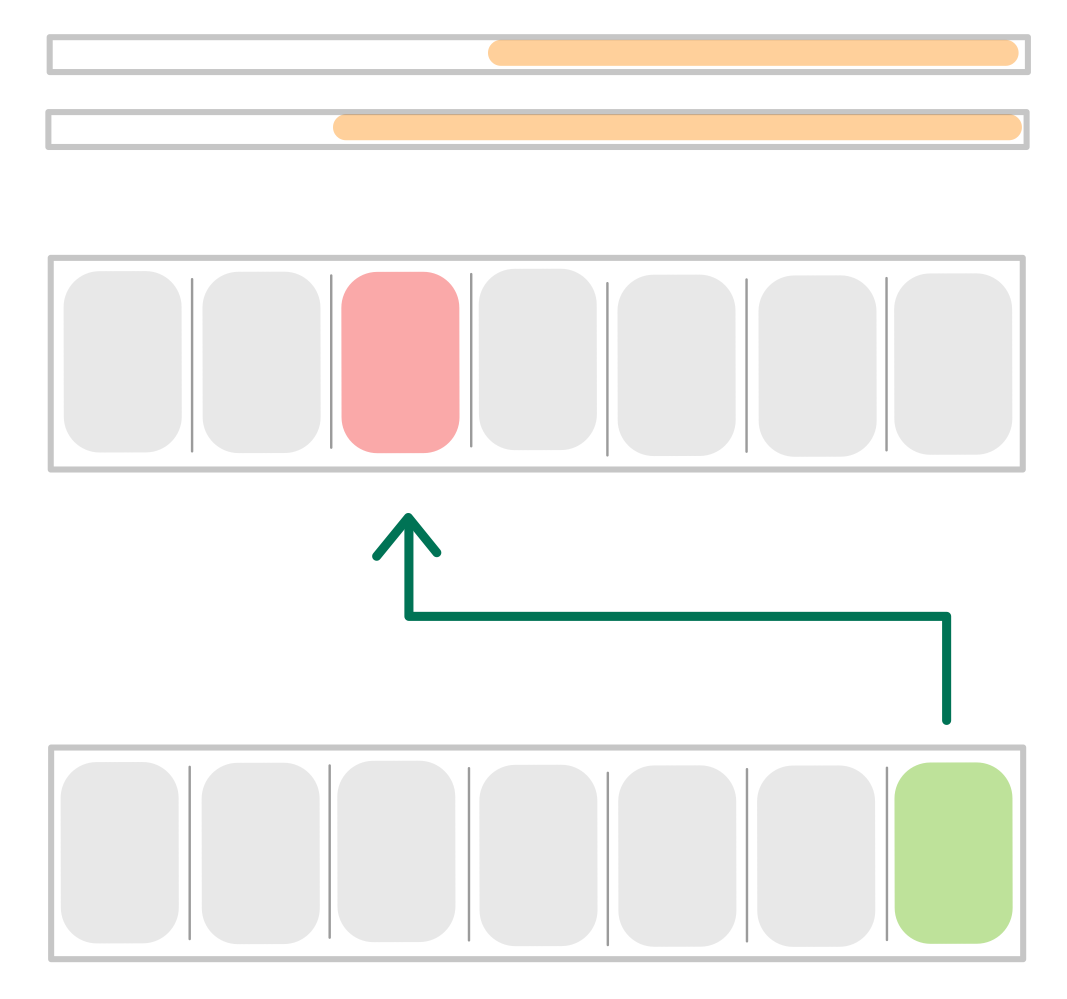
\includegraphics[width = 0.4\textwidth]{drawing/byte_swap}
\label{fig: one partial to one padded}
\caption{Representation of the constraints implemented by $\byteSwap$.}
\end{figure}